\section{سوال پنجم}

فرض کنید یک منبع با حجم نامحدودی از اطلاعات برای ارسال، از یک کنترل حلقه بسته (\lr{closed-loop control}) استفاده می‌کند تا نرخ ارسال خود را براساس اطلاعات بازخورد (\lr{feedback}) تنظیم کند. در صورتی که اطلاعات بازخورد نشان دهد هیچ ترافیکی (\lr{traffic}) در مسیر وجود ندارد، منبع به‌صورت پیوسته نرخ ارسال خود را به‌صورت خطی (\lr{linear}) افزایش می‌دهد. اما اگر اطلاعات بازخورد حاکی از وجود ترافیک در مسیر باشد، منبع نرخ ارسال را به صفر کاهش می‌دهد و سپس این چرخه را با افزایش تدریجی نرخ ارسال ادامه می‌دهد تا بار دیگر ترافیک شناسایی شود. حال فرض کنید که مدت زمانی معادل $T$ ثانیه طول می‌کشد تا اطلاعات بازخورد پس از وقوع ترافیک به منبع برسد. نمودار نرخ ارسال منبع را نسبت به زمان برای مقادیر کوچک و بزرگ $T$ ترسیم کنید و توضیح دهید که تأخیر انتشار $T$ \lr{(Propagation Delay)} چه نقشی در این کنترل حلقه بسته ایفا می‌کند.


\begin{qsolve}
	در این مسئله، یک منبع با استفاده از کنترل حلقه بسته نرخ ارسال خود را بر اساس اطلاعات بازخورد تنظیم می‌کند. رفتار منبع به صورت زیر توصیف می‌شود:
	
	\begin{itemize}
		\item \textbf{افزایش نرخ خطی در نبود ترافیک:}  
		در صورتی که هیچ ترافیکی شناسایی نشود، نرخ ارسال منبع به صورت خطی افزایش می‌یابد:
		\[
		R(t) = k \cdot t \quad \text{برای \( t \) پس از بازنشانی نرخ}
		\]
		که در آن \( k \) شیب افزایش نرخ ارسال است.
		
		\item \textbf{بازخورد ترافیک:}  
		وقتی ترافیک شناسایی شود (بر اساس اطلاعات بازخورد که بعد از تأخیر $T$ به منبع می‌رسد)، نرخ ارسال ناگهان به صفر کاهش می‌یابد. پس از این، منبع دوباره نرخ را از صفر شروع به افزایش می‌کند.
		
		
	\end{itemize}
	
	
	\begin{enumerate}
		\item \textbf{{نقش تأخیر \( T \)}}
		\begin{itemize}
			\item \textbf{مقادیر کوچک \( T \):}  
			در صورتی که تأخیر بازخورد $T$ کوچک باشد، منبع سریعاً از وجود ترافیک مطلع شده و نرخ ارسال را متناسب با بازخورد به صفر کاهش می‌دهد. این باعث می‌شود که نوسانات در نرخ ارسال کمتر باشد و شبکه پایدارتری داشته باشیم.
			
			\item \textbf{مقادیر بزرگ \( T \):}  
			اگر $T$ بزرگ باشد، منبع به مدت بیشتری نرخ ارسال را افزایش می‌دهد حتی پس از بروز ترافیک. در نتیجه، نرخ ارسال به مقادیر بالاتری می‌رسد پیش از اینکه بازخورد ترافیک دریافت شود و نرخ ناگهان به صفر کاهش یابد. این می‌تواند به نوسانات شدید در نرخ ارسال و احتمالا بارگذاری بیش‌ازحد شبکه منجر شود.
		\end{itemize}
		
		
		\item \textbf{{نمودار نرخ ارسال (\( R(t) \)) نسبت به زمان (\( t \))}}
		در شکل «\ref{fig:rate_comparison}»، نمودار نرخ ارسال منبع برای مقادیر کوچک و بزرگ \( T \) رسم شده است.
		
		
		نمودارها نشان می‌دهند که تأخیر بازخورد \( T \) تأثیر زیادی بر رفتار کنترل حلقه بسته دارد:
		\begin{itemize}
			\item تأخیر کوچک \( T \) منجر به نوسانات کوچک‌تر در نرخ ارسال و شبکه‌ای پایدارتر می‌شود.
			\item تأخیر بزرگ \( T \) باعث افزایش نوسانات و احتمال تراکم بیش از حد در شبکه می‌گردد.
		\end{itemize}
		
		
		
	\end{enumerate}
\end{qsolve}

\begin{figure}[h!]
	\centering
	\begin{subfigure}[b]{0.45\textwidth}
		\centering
		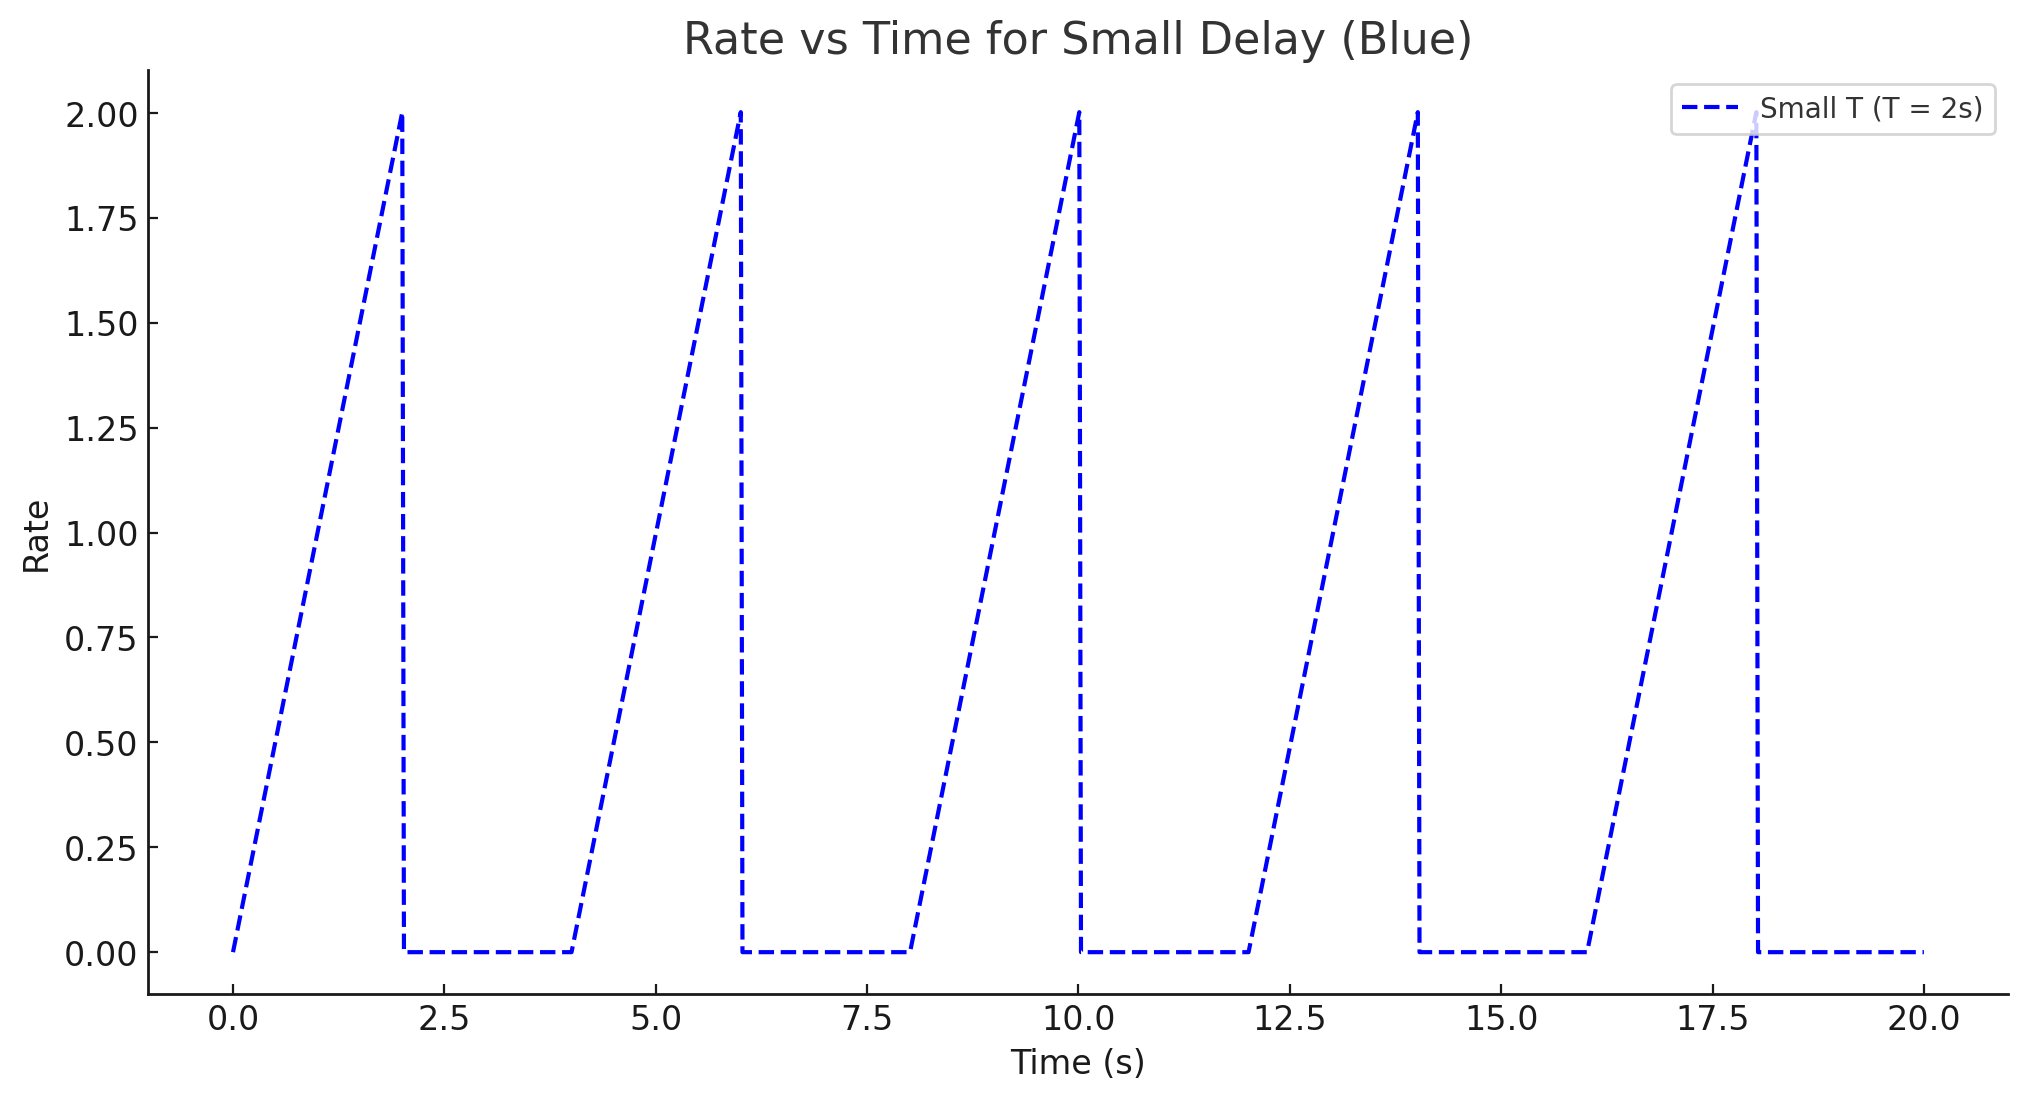
\includegraphics[width=\textwidth]{pics/img2.png}
		\caption{نمودار نرخ ارسال برای تأخیر کوچک (\( T = 2 \))}
		\label{fig:small_T}
	\end{subfigure}
	\hfill
	\begin{subfigure}[b]{0.45\textwidth}
		\centering
		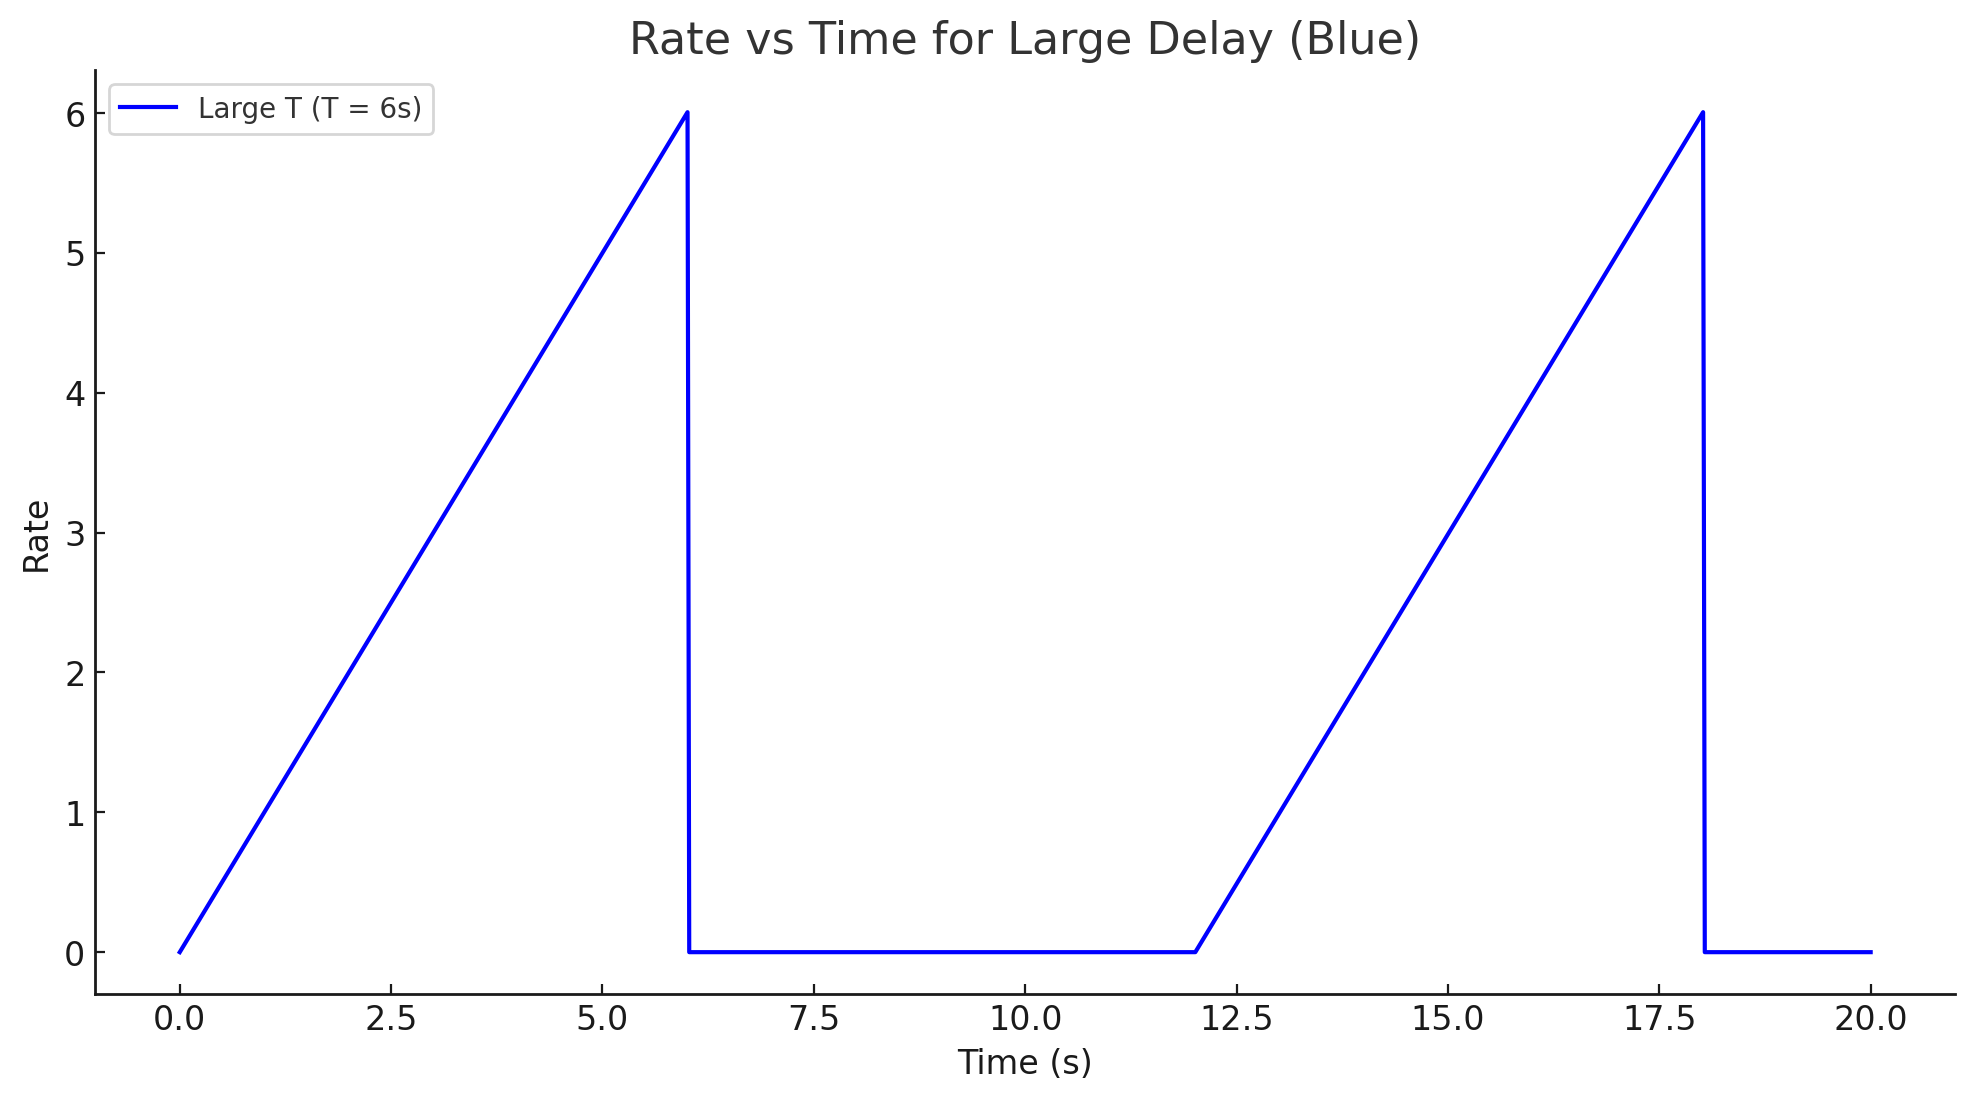
\includegraphics[width=\textwidth]{pics/img3.png}
		\caption{نمودار نرخ ارسال برای تأخیر بزرگ (\( T = 6 \))}
		\label{fig:large_T}
	\end{subfigure}
	\caption{مقایسه نرخ ارسال منبع برای مقادیر مختلف تأخیر \( T \)}
	\label{fig:rate_comparison}
\end{figure}